\chapter{Electronegatividad, polaridad y fuerzas intermoleculares}\label{ch:g11:polarity-and-cohesion}

Un geco sube por el cristal de una ventana y se queda colgado del vidrio
por un solo dedo, sin pegamento ni ventosa. Una \omterm{def:g7:atoms-and-molecules:molecule}{molécula} de agua,
\ce{H2O}, es más ligera que una \omterm{def:g7:atoms-and-molecules:molecule}{molécula} de sulfuro de hidrógeno,
\ce{H2S}, y sin embargo el agua hierve a \qty{100}{\celsius}, mientras
que el sulfuro de hidrógeno es un gas hasta \qty{-60}{\celsius}. Las dos
historias tratan de lo mismo: las fuerzas que mantienen unidas las
\omterm{def:g7:atoms-and-molecules:molecule}{moléculas} entre sí, y a otras cosas. Son mucho más débiles que los
\omterm{def:g10:lewis-and-shape:covalent-bond}{enlaces covalentes} del interior de una \omterm{def:g7:atoms-and-molecules:molecule}{molécula}, pero deciden si una
sustancia es un gas, un líquido o un sólido a temperatura ambiente, y si
un geco se cae.

\begin{recall}
Un \omterm{def:g10:lewis-and-shape:covalent-bond}{enlace covalente} es un par de \omterm{def:g9:inside-the-atom:nucleus}{electrones} compartido por dos \omterm{def:g7:atoms-and-molecules:atom}{átomos};
las \omterm{def:g10:lewis-and-shape:lewis-structure}{estructuras de Lewis} muestran los \omterm{def:g10:lewis-and-shape:lone-pair}{pares enlazantes} y los \omterm{def:g10:lewis-and-shape:lone-pair}{pares no
enlazantes}, y los pares que rodean a un \omterm{def:g7:atoms-and-molecules:atom}{átomo} central deciden la forma
de una \omterm{def:g7:atoms-and-molecules:molecule}{molécula} (\cref{ch:g10:lewis-and-shape}). Los \omterm{def:g9:ions:ion}{iones} tienen carga;
en un sólido iónico, los \omterm{def:g9:ions:ion}{iones} positivos y negativos se atraen
(\cref{ch:g9:ions}).
\end{recall}

\begin{omfigure}
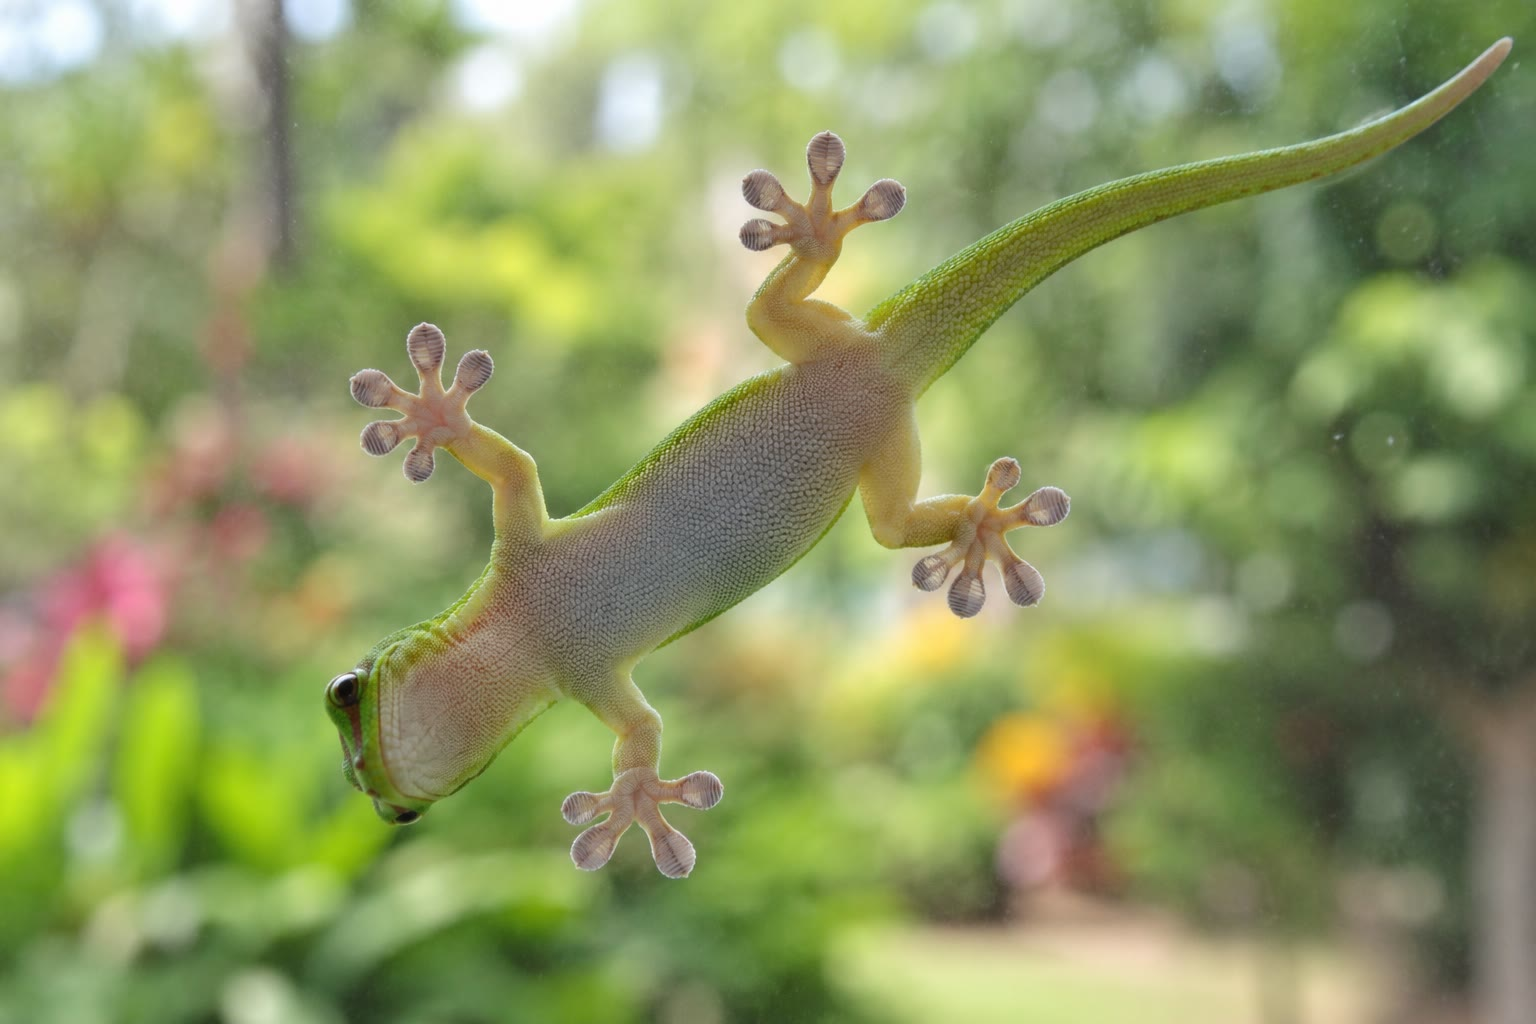
\includegraphics[width=0.5\linewidth]{images/book1/ai/g11-gecko-glass.jpg}

{\small Un geco sobre un cristal: las almohadillas de sus dedos se
sujetan gracias a fuerzas entre \omterm{def:g7:atoms-and-molecules:molecule}{moléculas}.}
\end{omfigure}

\section{La electronegatividad}

\begin{definition}[Electronegatividad]\label{def:g11:polarity-and-cohesion:electronegativity}
La \emph{electronegatividad}\index{electronegatividad} de un elemento
mide con qué fuerza atraen sus \omterm{def:g7:atoms-and-molecules:atom}{átomos}, en una \omterm{def:g7:atoms-and-molecules:molecule}{molécula}, los \omterm{def:g9:inside-the-atom:nucleus}{electrones}
de los enlaces que comparten. Es un número sin unidad; en la escala
habitual va de alrededor de 0.8 a alrededor de 4.
\end{definition}

\begin{omfigure}
% ledger: en:H, en:Li, en:Be, en:B, en:C, en:N, en:O, en:F, en:Na, en:Mg, en:Al, en:Si, en:P, en:S, en:Cl, en:K, en:Ca
\omperiodictable[upto=20, f block=false, cell=0.9cm, values={H/2.20,
  Li/0.98, Be/1.57, B/2.04, C/2.55, N/3.04, O/3.44, F/3.98, Na/0.93,
  Mg/1.31, Al/1.61, Si/1.90, P/2.19, S/2.58, Cl/3.16, K/0.82, Ca/1.00},
  highlight={F,O,N,Cl}]

{\small \omterm{def:g11:polarity-and-cohesion:electronegativity}{Electronegatividades} de los veinte primeros elementos (escala de
Pauling; no se da ninguna para el helio, el neón y el argón, que aquí no
forman enlaces). Resaltados: los cuatro más electronegativos.}
\end{omfigure}

\begin{proposition}[Tendencias en la tabla]\label{prop:g11:polarity-and-cohesion:trends}
% ledger: en:F, en:Li, en:Cl, en:K
La \omterm{def:g11:polarity-and-cohesion:electronegativity}{electronegatividad} aumenta de izquierda a derecha a lo largo de un
periodo y disminuye de arriba abajo en un grupo. El flúor (3.98) es el
elemento más electronegativo; los \omterm{def:g10:electron-shells:family}{metales alcalinos}, los menos (litio
0.98, potasio 0.82).
\end{proposition}

\begin{proof}
Se lee en la tabla: a lo largo del periodo 2, $0.98 < 1.57 < 2.04 < 2.55 < 3.04 <
3.44 < 3.98$; bajando por el \omterm{def:g9:periodic-table-first-look:period}{grupo} 17, el flúor, $3.98$, está por encima
del cloro, $3.16$; bajando por el \omterm{def:g9:periodic-table-first-look:period}{grupo} 1, $2.20$, $0.98$, $0.93$,
$0.82$. (Por qué es así se explica en el volumen del primer año
universitario.)
\end{proof}

\begin{history}[La escala de Pauling, 1932]
El químico Linus Pauling construyó la primera escala de
\omterm{def:g11:polarity-and-cohesion:electronegativity}{electronegatividad} en 1932, a partir de las energías de los enlaces
entre \omterm{def:g7:atoms-and-molecules:atom}{átomos} distintos. Dio al flúor el valor más alto, y la escala que
se usa en este capítulo sigue llevando su nombre.
\end{history}

\section{Enlaces polares y moléculas polares}

\begin{definition}[Enlace polar, carga parcial]\label{def:g11:polarity-and-cohesion:polar-bond}
Un \omterm{def:g10:lewis-and-shape:covalent-bond}{enlace covalente} entre dos \omterm{def:g7:atoms-and-molecules:atom}{átomos} de \omterm{def:g11:polarity-and-cohesion:electronegativity}{electronegatividades} distintas
es un \emph{enlace polar}\index{enlace polar}: el par compartido está
más cerca del \omterm{def:g7:atoms-and-molecules:atom}{átomo} más electronegativo. Ese \omterm{def:g7:atoms-and-molecules:atom}{átomo} lleva una pequeña
\emph{carga parcial}\index{carga parcial} negativa, que se escribe
$\delta^-$, y el otro \omterm{def:g7:atoms-and-molecules:atom}{átomo} una carga parcial positiva igual,
$\delta^+$.
\end{definition}

\begin{proposition}[¿Cuándo es polar un enlace?]\label{prop:g11:polarity-and-cohesion:polar-bond}
% ledger: en:C, en:H, en:O, en:Na, en:Cl
Un enlace entre dos \omterm{def:g7:atoms-and-molecules:atom}{átomos} idénticos no es polar. Entre \omterm{def:g7:atoms-and-molecules:atom}{átomos}
distintos, cuanto mayor es la diferencia de \omterm{def:g11:polarity-and-cohesion:electronegativity}{electronegatividades}, más
polar es el enlace; como regla práctica, una diferencia inferior a unos
0.4 (como \ce{C-H}, $2.55 - 2.20 = 0.35$) se considera apolar. Cuando la
diferencia es muy grande (como entre Na y Cl, $3.16 - 0.93 = 2.23$), los
\omterm{def:g9:inside-the-atom:nucleus}{electrones} no se comparten sino que se transfieren: el compuesto es
iónico.
\end{proposition}

\begin{proof}
Se admite: se deduce de la definición de la \omterm{def:g11:polarity-and-cohesion:electronegativity}{electronegatividad}, y los
umbrales son convenios.
\end{proof}

\begin{definition}[Moléculas polares y apolares]\label{def:g11:polarity-and-cohesion:polar-molecule}
Una \omterm{def:g7:atoms-and-molecules:molecule}{molécula} es una \emph{molécula polar}\index{molecula polar@molécula polar} si el
centro de sus \omterm{def:g11:polarity-and-cohesion:polar-bond}{cargas parciales} positivas y el centro de sus \omterm{def:g11:polarity-and-cohesion:polar-bond}{cargas
parciales} negativas no coinciden; si coinciden, es una
\emph{molécula apolar}\index{molecula apolar@molécula apolar}.
\end{definition}

\begin{method}[¿Es polar una molécula?]\label{met:g11:polarity-and-cohesion:polar}
\begin{enumerate}
  \item Dibujar la \omterm{def:g10:lewis-and-shape:lewis-structure}{estructura de Lewis} y hallar la forma de la \omterm{def:g7:atoms-and-molecules:molecule}{molécula}.
  \item Marcar los \omterm{def:g11:polarity-and-cohesion:polar-bond}{enlaces polares} con $\delta^+$ y $\delta^-$.
  \item Si no hay ningún \omterm{def:g11:polarity-and-cohesion:polar-bond}{enlace polar}, la \omterm{def:g7:atoms-and-molecules:molecule}{molécula} es apolar. Si no,
        fijarse en la forma: si los \omterm{def:g11:polarity-and-cohesion:polar-bond}{enlaces polares} están dispuestos de
        forma simétrica alrededor del centro, sus efectos se anulan y la
        \omterm{def:g7:atoms-and-molecules:molecule}{molécula} es apolar; si no, es polar.
\end{enumerate}
\end{method}

\begin{omfigure}
\begin{tikzpicture}[font=\small]
  % water
  \begin{scope}
    \node[aO] (o) at (0,0) {};
    \node[aH] (h1) at (-0.82,-0.6) {};
    \node[aH] (h2) at (0.82,-0.6) {};
    \begin{scope}[on background layer]
      \draw[bond] (o.center) -- (h1.center); \draw[bond] (o.center) -- (h2.center);
    \end{scope}
    \node[omThm] at (0,0.55) {$2\delta^-$};
    \node[omDef] at (-1.22,-0.5) {$\delta^+$};
    \node[omDef] at (1.22,-0.5) {$\delta^+$};
    \fill[omDef] (0,-0.6) circle (0.06);
    \fill[omThm] (0,0) circle (0.06);
    \draw[densely dotted, black!60] (-0.82,-0.6) -- (0.82,-0.6);
    \draw[<-, black!60] (0.08,-0.64) -- (1.55,-1.05) node[right, align=left,
      font=\footnotesize] {centro de\\ los $\delta^+$};
    \node[align=center, anchor=north] at (0,-1.8) {agua: angular, \textbf{polar}};
  \end{scope}
  % carbon dioxide
  \begin{scope}[xshift=6cm]
    \node[aO] (o1) at (-1.15,0) {};
    \node[aC] (c) at (0,0) {};
    \node[aO] (o2) at (1.15,0) {};
    \begin{scope}[on background layer]
      \draw[bond, double, double distance=1.6pt] (o1.center) -- (c.center);
      \draw[bond, double, double distance=1.6pt] (c.center) -- (o2.center);
    \end{scope}
    \node[omThm] at (-1.15,0.55) {$\delta^-$};
    \node[omThm] at (1.15,0.55) {$\delta^-$};
    \node[omDef] at (0,0.55) {$2\delta^+$};
    \draw[->, omProp, thick] (-0.25,-0.45) -- (-1.0,-0.45);
    \draw[->, omProp, thick] (0.25,-0.45) -- (1.0,-0.45);
    \node[align=center, anchor=north] at (0,-1.8) {dióxido de carbono: lineal,\\
      \textbf{apolar}};
  \end{scope}
\end{tikzpicture}

{\small En el agua, la forma angular sitúa el centro de las \omterm{def:g11:polarity-and-cohesion:polar-bond}{cargas
parciales} positivas (entre los \omterm{def:g7:atoms-and-molecules:atom}{átomos} de hidrógeno) por debajo del
\omterm{def:g7:atoms-and-molecules:atom}{átomo} de oxígeno: la \omterm{def:g7:atoms-and-molecules:molecule}{molécula} es polar. En el dióxido de carbono, los
dos \omterm{def:g11:polarity-and-cohesion:polar-bond}{enlaces polares} tiran en sentidos opuestos (flechas) y se anulan:
los centros de carga coinciden en el \omterm{def:g7:atoms-and-molecules:atom}{átomo} de carbono.}
\end{omfigure}


\begin{example}[Cuatro moléculas]\label{ex:g11:polarity-and-cohesion:four}
El cloruro de hidrógeno \ce{HCl} tiene un \omterm{def:g11:polarity-and-cohesion:polar-bond}{enlace polar} y es polar, con
el cloro $\delta^-$. El amoniaco \ce{NH3}, una pirámide de tres \omterm{def:g11:polarity-and-cohesion:polar-bond}{enlaces
polares} \ce{N-H}, es polar, con el nitrógeno $\delta^-$. El metano
\ce{CH4} solo tiene enlaces \ce{C-H} casi apolares: es apolar. El
tetraclorometano \ce{CCl4} tiene cuatro \omterm{def:g11:polarity-and-cohesion:polar-bond}{enlaces polares} \ce{C-Cl}, pero
en los vértices de un tetraedro regular: sus efectos se anulan y la
\omterm{def:g7:atoms-and-molecules:molecule}{molécula} es apolar.
\end{example}

\section{Las interacciones de van der Waals}

\begin{definition}[Interacción de van der Waals]\label{def:g11:polarity-and-cohesion:van-der-waals}
Una \emph{interacción de van der Waals}\index{interaccion de van der Waals@interacción de van der Waals}
es una atracción débil entre \omterm{def:g7:atoms-and-molecules:molecule}{moléculas} vecinas, que existe entre todas
las \omterm{def:g7:atoms-and-molecules:molecule}{moléculas}, polares o no: los \omterm{def:g9:inside-the-atom:nucleus}{electrones} de cada \omterm{def:g7:atoms-and-molecules:molecule}{molécula} se mueven
sin cesar, y las cargas desiguales momentáneas de una \omterm{def:g7:atoms-and-molecules:molecule}{molécula} atraen a
las de sus vecinas. Entre \omterm{def:g11:polarity-and-cohesion:polar-molecule}{moléculas polares}, las \omterm{def:g11:polarity-and-cohesion:polar-bond}{cargas parciales}
permanentes añaden una atracción más.
\end{definition}


\begin{proposition}[Las moléculas más grandes se atraen más]\label{prop:g11:polarity-and-cohesion:size}
Las \omterm{def:g11:polarity-and-cohesion:van-der-waals}{interacciones de van der Waals} crecen con el tamaño de las
\omterm{def:g7:atoms-and-molecules:molecule}{moléculas}, es decir, con su número de \omterm{def:g9:inside-the-atom:nucleus}{electrones}; entre \omterm{def:g7:atoms-and-molecules:molecule}{moléculas}
parecidas, las más grandes tienen las temperaturas de fusión y de
ebullición más altas.
\end{proposition}

\begin{proof}
Se admite: una nube electrónica más grande se deforma con más
facilidad, así que sus cargas momentáneas son mayores, y tiene más
contacto con sus vecinas.
\end{proof}

\begin{example}[Los halógenos]\label{ex:g11:polarity-and-cohesion:halogens}
% ledger: bp:F2, bp:Cl2, bp:Br2, bp:I2 (K values converted)
Las \omterm{def:g7:atoms-and-molecules:molecule}{moléculas} \ce{F2}, \ce{Cl2}, \ce{Br2}, \ce{I2} son todas apolares y
cada vez más grandes. Sus temperaturas de ebullición suben con ellas:
\qty{-188}{\celsius}, \qty{-34}{\celsius}, \qty{59}{\celsius} y
\qty{184}{\celsius}. A temperatura ambiente, el flúor y el cloro son
gases, el bromo es líquido y el yodo, sólido.
\end{example}

\begin{remark}[El geco]\label{rem:g11:polarity-and-cohesion:gecko}
Una sola \omterm{def:g11:polarity-and-cohesion:van-der-waals}{interacción de van der Waals} es minúscula, pero se suman. Las
almohadillas de los dedos de un geco están cubiertas de una densa
alfombra de pelos microscópicos, cada uno dividido en puntas aún más
finas, que se acercan lo suficiente al vidrio para que las \omterm{def:g11:polarity-and-cohesion:van-der-waals}{interacciones
de van der Waals} actúen sobre una superficie total muy grande.
\end{remark}

\section{Los enlaces de hidrógeno}

\begin{definition}[Enlace de hidrógeno]\label{def:g11:polarity-and-cohesion:hydrogen-bond}
Un \emph{enlace de hidrógeno}\index{enlace de hidrogeno@enlace de hidrógeno} es una
atracción entre un \omterm{def:g7:atoms-and-molecules:atom}{átomo} de hidrógeno unido a un \omterm{def:g7:atoms-and-molecules:atom}{átomo} muy
electronegativo (nitrógeno, oxígeno o flúor), que lleva un $\delta^+$
marcado, y un \omterm{def:g10:lewis-and-shape:lone-pair}{par no enlazante} de otro \omterm{def:g7:atoms-and-molecules:atom}{átomo} de nitrógeno, oxígeno o
flúor, a menudo de una \omterm{def:g7:atoms-and-molecules:molecule}{molécula} vecina. Se dibuja con una línea
discontinua, y los tres \omterm{def:g7:atoms-and-molecules:atom}{átomos} implicados están casi en línea recta.
\end{definition}

\begin{omfigure}
\begin{tikzpicture}[font=\small]
  % central water molecule and four neighbours, H-bonds dashed
  \newcommand{\water}[4]{% name, x, y, rotation
    \begin{scope}[shift={(#2,#3)}, rotate=#4]
      \node[aO] (#1o) at (0,0) {};
      \node[aH] (#1a) at (-0.6,-0.45) {};
      \node[aH] (#1b) at (0.6,-0.45) {};
    \end{scope}
    \begin{scope}[on background layer]
      \draw[bond] (#1o.center) -- (#1a.center); \draw[bond] (#1o.center) -- (#1b.center);
    \end{scope}}
  \water{m}{0}{0}{0}
  \water{p}{-1.62}{-1.215}{0}
  \water{q}{1.62}{-1.215}{0}
  \water{r}{-1.435}{1.435}{-8.13}
  \water{s}{1.435}{1.435}{8.13}
  % H-bonds: m's H to p's O and q's O; r's and s's H to m's O
  \draw[dashed, omDef, thick] (ma) -- (po);
  \draw[dashed, omDef, thick] (mb) -- (qo);
  \draw[dashed, omDef, thick] (rb) -- (mo);
  \draw[dashed, omDef, thick] (sa) -- (mo);
\end{tikzpicture}

{\small \omterm{def:g11:polarity-and-cohesion:hydrogen-bond}{Enlaces de hidrógeno} (discontinuos) alrededor de una \omterm{def:g7:atoms-and-molecules:molecule}{molécula} de
agua en el agua líquida: sus dos \omterm{def:g7:atoms-and-molecules:atom}{átomos} de hidrógeno se unen a los
\omterm{def:g7:atoms-and-molecules:atom}{átomos} de oxígeno de dos vecinas, y los dos \omterm{def:g10:lewis-and-shape:lone-pair}{pares no enlazantes} de su
\omterm{def:g7:atoms-and-molecules:atom}{átomo} de oxígeno reciben los \omterm{def:g7:atoms-and-molecules:atom}{átomos} de hidrógeno de otras dos.}
\end{omfigure}


\begin{example}[El etanol y el propano]\label{ex:g11:polarity-and-cohesion:ethanol}
% ledger: bp:C2H5OH, bp:C3H8 (K values converted)
El etanol, \ce{CH3-CH2-OH} (\qty{46.0}{g/mol}), y el propano,
\ce{CH3-CH2-CH3} (\qty{44.0}{g/mol}), tienen \omterm{def:g7:atoms-and-molecules:molecule}{moléculas} de casi el mismo
tamaño. Sin embargo, el etanol hierve a \qty{78}{\celsius} y el propano
a \qty{-42}{\celsius}. Las \omterm{def:g7:atoms-and-molecules:molecule}{moléculas} de etanol, con su grupo \ce{O-H},
forman \omterm{def:g11:polarity-and-cohesion:hydrogen-bond}{enlaces de hidrógeno} entre sí; las de propano no pueden.
\end{example}

\section{La cohesión de los sólidos y de los líquidos}

\begin{definition}[Sólido molecular]\label{def:g11:polarity-and-cohesion:molecular-solid}
Un \emph{sólido molecular}\index{solido molecular@sólido molecular} es un sólido formado
por \omterm{def:g7:atoms-and-molecules:molecule}{moléculas} unidas entre sí por \omterm{def:g11:polarity-and-cohesion:van-der-waals}{interacciones de van der Waals} y,
cuando es posible, por \omterm{def:g11:polarity-and-cohesion:hydrogen-bond}{enlaces de hidrógeno}. El hielo, el yodo sólido y
el azúcar son sólidos moleculares.
\end{definition}

\begin{proposition}[Cohesión y cambio de estado]\label{prop:g11:polarity-and-cohesion:cohesion}
Cuanto más fuertes son las atracciones entre las partículas de una
sustancia, más altas son sus temperaturas de fusión y de ebullición. Por
orden creciente de intensidad: las \omterm{def:g11:polarity-and-cohesion:van-der-waals}{interacciones de van der Waals}, los
\omterm{def:g11:polarity-and-cohesion:hydrogen-bond}{enlaces de hidrógeno} y la atracción entre los \omterm{def:g9:ions:ion}{iones} de un sólido
iónico.
\end{proposition}

\begin{proof}
Se admite: fundir y hervir separan las partículas venciendo esas
atracciones, lo que necesita más energía, y por tanto una temperatura
más alta, cuando son más fuertes.
\end{proof}

\begin{example}[Tres sólidos]\label{ex:g11:polarity-and-cohesion:three}
% ledger: mp:NaCl, mp:water
El cloruro de sodio, un sólido iónico, funde a \qty{801}{\celsius}; el
hielo, unido por \omterm{def:g11:polarity-and-cohesion:hydrogen-bond}{enlaces de hidrógeno}, a \qty{0}{\celsius}; el metano
sólido, unido solo por \omterm{def:g11:polarity-and-cohesion:van-der-waals}{interacciones de van der Waals} entre \omterm{def:g7:atoms-and-molecules:molecule}{moléculas}
pequeñas, muy por debajo de \qty{-150}{\celsius}.
\end{example}

\begin{omfigure}
\begin{tikzpicture}
\begin{axis}[width=0.6\linewidth, height=7cm, xmin=1.7, xmax=5.3,
    ymin=-190, ymax=120, xtick={2,3,4,5}, xlabel={periodo},
    ylabel={temperatura de ebullición (\si{\celsius})}, axis lines*=left,
    ymajorgrids, grid style={gray!20}, tick label style={font=\small},
    label style={font=\small},
    legend style={font=\small, at={(1.02,0.5)}, anchor=west, draw=none},
    legend cell align=left]
  % ledger: bp:CH4, bp:SiH4, bp:GeH4, bp:NH3, bp:PH3, bp:AsH3, bp:SbH3, bp:H2O, bp:H2S, bp:H2Se, bp:HF, bp:HCl, bp:HBr, bp:HI (K values converted to degC)
  \addplot[thick, mark=*, black!70] coordinates {(2,-162.2) (3,-112) (4,-88.1)};
  \addplot[thick, mark=square*, omMeth] coordinates {(2,-33.4) (3,-87.8) (4,-62.5) (5,-18.4)};
  \addplot[thick, mark=triangle*, mark size=3pt, omThm] coordinates {(2,100.0) (3,-60.3) (4,-41.3)};
  \addplot[thick, mark=diamond*, mark size=3pt, omDef] coordinates {(2,19.6) (3,-85.1) (4,-66.4) (5,-35.1)};
  \legend{grupo 14 (\ce{CH4} \dots), grupo 15 (\ce{NH3} \dots),
    grupo 16 (\ce{H2O} \dots), grupo 17 (\ce{HF} \dots)}
  \node[font=\footnotesize, anchor=west] at (axis cs:2.05,100) {\ce{H2O}};
  \node[font=\footnotesize, anchor=west] at (axis cs:2.05,19.6) {\ce{HF}};
  \node[font=\footnotesize, anchor=west] at (axis cs:2.05,-33.4) {\ce{NH3}};
  \node[font=\footnotesize, anchor=north west] at (axis cs:2.05,-166) {\ce{CH4}};
\end{axis}
\end{tikzpicture}

{\small Temperaturas de ebullición de los compuestos del hidrógeno con
los elementos de los \omterm{def:g9:periodic-table-first-look:period}{grupos} 14 a 17. En cada grupo suben con el tamaño
de la \omterm{def:g7:atoms-and-molecules:molecule}{molécula}, salvo para el primer miembro de los \omterm{def:g9:periodic-table-first-look:period}{grupos} 15, 16 y 17,
demasiado alto: el amoniaco, el agua y el fluoruro de hidrógeno forman
\omterm{def:g11:polarity-and-cohesion:hydrogen-bond}{enlaces de hidrógeno}. (No se representa ningún valor allí donde las
fuentes utilizadas no lo dan.)}
\end{omfigure}

\begin{remark}[Hielo y nieve]\label{rem:g11:polarity-and-cohesion:ice}
En el hielo, cada \omterm{def:g7:atoms-and-molecules:molecule}{molécula} de agua está unida por \omterm{def:g11:polarity-and-cohesion:hydrogen-bond}{enlaces de hidrógeno} a
cuatro vecinas, en una red abierta de anillos hexagonales. Esa red deja
más espacio vacío que el agua líquida, donde los enlaces se rompen y se
vuelven a formar sin cesar: el hielo es menos denso que el agua y
flota. La simetría de orden seis de los cristales de nieve refleja los
anillos hexagonales de la red.
\end{remark}

\begin{omfigure}
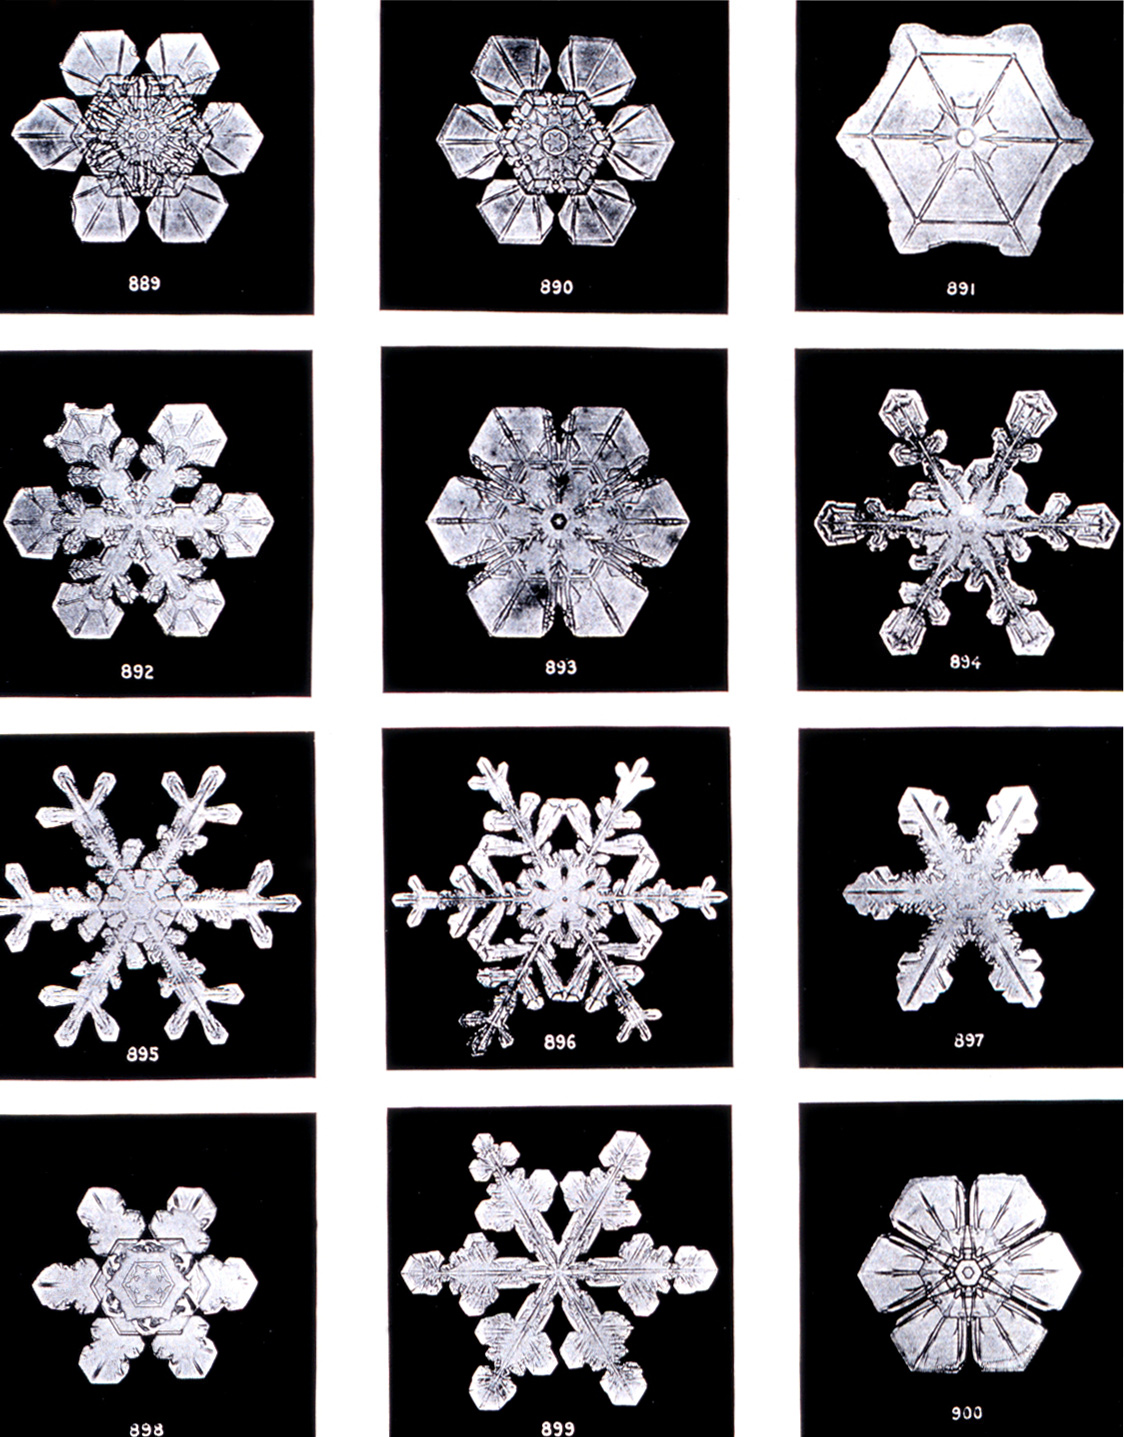
\includegraphics[width=0.36\linewidth]{images/book1/snowflakes.jpg}

{\small Cristales de nieve fotografiados por Wilson Bentley a principios
del siglo XX: todos tienen seis brazos.}
\end{omfigure}

\section{Ejercicios}


\begin{exercise}[$\star$]\label{exo:g11:polarity-and-cohesion:1}
En los enlaces \ce{H-Cl}, \ce{O-H} y \ce{C-O}, ¿qué \omterm{def:g7:atoms-and-molecules:atom}{átomo} lleva la
\omterm{def:g11:polarity-and-cohesion:polar-bond}{carga parcial} $\delta^-$? Usa la tabla de \omterm{def:g11:polarity-and-cohesion:electronegativity}{electronegatividades}.
\end{exercise}

\begin{exercise}[$\star$]\label{exo:g11:polarity-and-cohesion:2}
¿Cuáles de estos enlaces son polares: \ce{H-H}, \ce{C-H}, \ce{O-H},
\ce{N-H}, \ce{Cl-Cl}, \ce{C-Cl}? Da la diferencia de \omterm{def:g11:polarity-and-cohesion:electronegativity}{electronegatividades}
de cada uno.
\end{exercise}

\begin{exercise}[$\star$]\label{exo:g11:polarity-and-cohesion:3}
¿Qué elemento es más electronegativo en cada pareja: el nitrógeno o el
fósforo; el oxígeno o el azufre; el carbono o el nitrógeno; el sodio o
el magnesio? ¿Qué tendencia de la tabla ilustra cada pareja?
\end{exercise}

\begin{exercise}[$\star$]\label{exo:g11:polarity-and-cohesion:4}
¿Cuáles de \ce{CH4}, \ce{NH3}, \ce{H2O} y \ce{HCl} pueden formar \omterm{def:g11:polarity-and-cohesion:hydrogen-bond}{enlaces
de hidrógeno} entre sus propias \omterm{def:g7:atoms-and-molecules:molecule}{moléculas}? Explícalo.
\end{exercise}

\begin{exercise}[$\star$]\label{exo:g11:polarity-and-cohesion:5}
¿Hay alguna atracción entre las \omterm{def:g11:polarity-and-cohesion:polar-molecule}{moléculas apolares} del metano? ¿Por qué
el metano es, aun así, un gas a temperatura ambiente?
\end{exercise}

\begin{exercise}[$\star\star$]\label{exo:g11:polarity-and-cohesion:6}
Di si cada \omterm{def:g7:atoms-and-molecules:molecule}{molécula} es polar: el diclorometano \ce{CH2Cl2}
(tetraédrico), el tetraclorometano \ce{CCl4}, el amoniaco \ce{NH3}, el
dióxido de carbono \ce{CO2}, el trifluoruro de boro \ce{BF3} (un
triángulo plano con el boro en el centro).
\end{exercise}

\begin{exercise}[$\star\star$]\label{exo:g11:polarity-and-cohesion:7}
En el metanol, \ce{CH3-OH}, ¿qué \omterm{def:g7:atoms-and-molecules:atom}{átomo} de hidrógeno se puede ceder en un
\omterm{def:g11:polarity-and-cohesion:hydrogen-bond}{enlace de hidrógeno}? ¿Qué \omterm{def:g7:atoms-and-molecules:atom}{átomo} puede recibir uno? ¿Pueden formar
\omterm{def:g11:polarity-and-cohesion:hydrogen-bond}{enlaces de hidrógeno} entre sí las \omterm{def:g7:atoms-and-molecules:molecule}{moléculas} de metanol y las de agua?
Dibuja uno.
\end{exercise}

\begin{exercise}[$\star\star$]\label{exo:g11:polarity-and-cohesion:8}
Explica por qué las temperaturas de ebullición suben en el orden
\ce{CH4} <
\ce{SiH4} < \ce{GeH4}.
\end{exercise}

\begin{exercise}[$\star\star$]\label{exo:g11:polarity-and-cohesion:9}
En el gráfico de las temperaturas de ebullición de los hidruros, ¿qué
grupo no presenta ningún valor anómalo para su primer miembro? ¿Por qué?
\end{exercise}

\begin{exercise}[$\star\star$]\label{exo:g11:polarity-and-cohesion:10}
% ledger: en:H, en:Cl, en:Br, en:I, bp:HCl, bp:HBr, bp:HI
Los enlaces \ce{H-Cl}, \ce{H-Br}, \ce{H-I} son cada vez menos polares
(las \omterm{def:g11:polarity-and-cohesion:electronegativity}{electronegatividades} del cloro, el bromo y el yodo son 3.16, 2.96 y
2.66) y, sin embargo, las temperaturas de ebullición suben:
\qty{-85}{\celsius}, \qty{-66}{\celsius}, \qty{-35}{\celsius}. ¿Qué
interacción gana, y por qué?
\end{exercise}

\begin{exercise}[$\star\star$]\label{exo:g11:polarity-and-cohesion:11}
A temperatura ambiente, el cloro es un gas y el yodo un sólido, aunque
los dos estén formados por \omterm{def:g11:polarity-and-cohesion:polar-molecule}{moléculas apolares} \ce{X2}. Explícalo.
\end{exercise}

\begin{exercise}[$\star\star\star$]\label{exo:g11:polarity-and-cohesion:12}
% ledger: bp:C2H5OH, bp:CH3OCH3, bp:C3H8
El etanol \ce{CH3-CH2-OH}, el metoximetano \ce{CH3-O-CH3} y el propano
\ce{CH3-CH2-CH3} tienen casi la misma \omterm{def:g10:the-mole:molar-mass}{masa molar}. Hierven a
\qty{78}{\celsius}, \qty{-25}{\celsius} y \qty{-42}{\celsius}. ¿Cuáles
son polares? ¿Cuáles forman \omterm{def:g11:polarity-and-cohesion:hydrogen-bond}{enlaces de hidrógeno} entre sus propias
\omterm{def:g7:atoms-and-molecules:molecule}{moléculas}? Explica el orden.
\end{exercise}

\begin{exercise}[$\star\star\star$]\label{exo:g11:polarity-and-cohesion:13}
En el hielo, cada \omterm{def:g7:atoms-and-molecules:molecule}{molécula} de agua está unida por \omterm{def:g11:polarity-and-cohesion:hydrogen-bond}{enlaces de hidrógeno} a
cuatro vecinas, en una red abierta; en el agua líquida, la red se rompe
sin cesar y se colapsa en parte. Explica por qué el hielo flota sobre el
agua. ¿Por qué es importante esto para los peces de un lago helado?
\end{exercise}

\begin{exercise}[$\star\star\star$]\label{exo:g11:polarity-and-cohesion:14}
Ordena por temperatura de fusión creciente, y justifícalo con las
atracciones entre las partículas: el cloruro de potasio \ce{KCl}, el
hielo \ce{H2O}, el metano sólido \ce{CH4}.
\end{exercise}

\begin{exercise}[$\star\star\star$]\label{exo:g11:polarity-and-cohesion:15}
% ledger: en:F, en:O, bp:HF, bp:H2O
El flúor es más electronegativo que el oxígeno, así que un enlace
\ce{H-F} es más polar que un enlace \ce{O-H}. Sin embargo, el agua
hierve a \qty{100}{\celsius} y el fluoruro de hidrógeno a
\qty{20}{\celsius}. Cuenta los \omterm{def:g7:atoms-and-molecules:atom}{átomos} de hidrógeno que puede ceder cada
\omterm{def:g7:atoms-and-molecules:molecule}{molécula} y los \omterm{def:g10:lewis-and-shape:lone-pair}{pares no enlazantes} con los que puede recibirlos, y
explícalo.
\end{exercise}

\section{Problema: ¿Por qué hierve el agua a \texorpdfstring{\qty{100}{\celsius}}{100 grados Celsius}?}

\begin{problem}[{Problema de fin de semana --- sin enlaces de hidrógeno,
¿a qué temperatura herviría el agua?}]
\label{pb:g11:polarity-and-cohesion:1}
% ledger: en:H, en:O, en:S, en:Se, bp:H2O, bp:H2S, bp:H2Se, bp:CH4, bp:SiH4, bp:GeH4, bp:HCl, bp:HBr, bp:HF, bp:NH3, bp:PH3, bp:AsH3
El oxígeno, el azufre y el selenio están en el mismo grupo de la tabla,
y los tres forman un compuesto con el hidrógeno: \ce{H2O}, \ce{H2S},
\ce{H2Se}. En cada grupo de hidruros, las temperaturas de ebullición
suelen subir con el tamaño de la \omterm{def:g7:atoms-and-molecules:molecule}{molécula}. El agua rompe la regla. ¿En
cuánto?

\medskip
\noindent\textbf{Parte I --- Tres \omterm{def:g7:atoms-and-molecules:molecule}{moléculas}.}
\begin{enumerate}
  \item Dibuja las \omterm{def:g10:lewis-and-shape:lewis-structure}{estructuras de Lewis} de \ce{H2O}, \ce{H2S} y
        \ce{H2Se}. ¿Por qué se parecen?
  \item Calcula sus \omterm{def:g10:the-mole:molar-mass}{masas molares}.
  \item Calcula las diferencias de \omterm{def:g11:polarity-and-cohesion:electronegativity}{electronegatividad} de los enlaces
        \ce{O-H}, \ce{S-H} y \ce{Se-H} (oxígeno 3.44, azufre 2.58,
        selenio 2.55, hidrógeno 2.20). ¿Qué enlaces son claramente
        polares?
  \item ¿Qué forma tienen las tres \omterm{def:g7:atoms-and-molecules:molecule}{moléculas}? ¿Son polares?
  \item Cuenta los \omterm{def:g9:inside-the-atom:nucleus}{electrones} de cada \omterm{def:g7:atoms-and-molecules:molecule}{molécula}. ¿Cuál tiene las
        \omterm{def:g11:polarity-and-cohesion:van-der-waals}{interacciones de van der Waals} más fuertes?
\end{enumerate}

\medskip
\noindent\textbf{Parte II --- Los \omterm{def:g11:polarity-and-cohesion:hydrogen-bond}{enlaces de hidrógeno}.}
\begin{enumerate}[resume]
  \item ¿Cuál de los tres compuestos forma \omterm{def:g11:polarity-and-cohesion:hydrogen-bond}{enlaces de hidrógeno} entre
        sus \omterm{def:g7:atoms-and-molecules:molecule}{moléculas}? ¿Por qué los otros no?
  \item ¿En cuántos \omterm{def:g11:polarity-and-cohesion:hydrogen-bond}{enlaces de hidrógeno} puede participar como mucho una
        \omterm{def:g7:atoms-and-molecules:molecule}{molécula} de agua? Dibújalos.
  \item ¿Qué interacciones mantienen unidas las \omterm{def:g7:atoms-and-molecules:molecule}{moléculas} del sulfuro de
        hidrógeno en el líquido?
\end{enumerate}

\medskip
\noindent\textbf{Parte III --- La tendencia.}
\begin{enumerate}[resume]
  \item El sulfuro de hidrógeno hierve a \qty{212.9}{K} y el seleniuro
        de hidrógeno a \qty{-41.3}{\celsius}. Expresa la primera en grados
        Celsius
        ($\theta = T - 273.15$).
  \item ¿Cuánto sube la temperatura de ebullición del periodo 3
        (\ce{H2S}) al periodo 4 (\ce{H2Se})?
  \item ¿Por qué sube?
  \item Suponiendo la misma subida del periodo 2 al periodo 3, ¿a qué
        temperatura herviría un \ce{H2O} ``normal''?
  \item Prueba el método con el \omterm{def:g9:periodic-table-first-look:period}{grupo} 14: el \ce{SiH4} hierve a
        \qty{-112}{\celsius} y el \ce{GeH4} a \qty{-88.1}{\celsius}.
        Predice la temperatura de ebullición del \ce{CH4} y compárala con
        la real, \qty{-162}{\celsius}. ¿Es exacta la extrapolación?
  \item Haz lo mismo con el \omterm{def:g9:periodic-table-first-look:period}{grupo} 17 (\ce{HCl} \qty{-85.1}{\celsius},
        \ce{HBr} \qty{-66.4}{\celsius}) y compara con el \ce{HF},
        \qty{19.6}{\celsius}.
\end{enumerate}

\medskip
\noindent\textbf{Parte IV --- La diferencia.}
\begin{enumerate}[resume]
  \item El agua hierve en realidad a \qty{100}{\celsius}. ¿Qué
        diferencia hay entre el valor real y el extrapolado?
  \item Lo mismo para el amoniaco, con \ce{PH3} \qty{-87.8}{\celsius} y
        \ce{AsH3} \qty{-62.5}{\celsius}; el amoniaco hierve en realidad
        a
        \qty{-33.4}{\celsius}.
  \item Ordena el agua, el fluoruro de hidrógeno y el amoniaco según el
        tamaño de su diferencia, y explica el orden contando \omterm{def:g11:polarity-and-cohesion:hydrogen-bond}{enlaces de
        hidrógeno}.
  \item Sin \omterm{def:g11:polarity-and-cohesion:hydrogen-bond}{enlaces de hidrógeno}, ¿sería el agua un sólido, un líquido o
        un gas a temperatura ambiente? ¿Qué supondría eso para la
        Tierra?
  \item ¿Por qué la respuesta a la pregunta 12 es solo una estimación?
  \item Da la respuesta final: ¿a qué temperatura, más o menos, herviría
        el agua sin \omterm{def:g11:polarity-and-cohesion:hydrogen-bond}{enlaces de hidrógeno}?
\end{enumerate}
\end{problem}
